%File: formatting-instruction.tex
\documentclass[letterpaper]{article}
\usepackage{aaai}

\usepackage{times}
\usepackage{helvet}
\usepackage{courier}
\usepackage{graphicx}
\usepackage{comment}
\usepackage{float}
\frenchspacing
\setlength{\pdfpagewidth}{8.5in}
\setlength{\pdfpageheight}{11in}
\pdfinfo{
/Title (DS5110 Project Report)
/Author (Ibrahim Byiringiro, Shushant Ghosh, Tianrui Chen)}
\setcounter{secnumdepth}{0}  
 \begin{document}
% The file aaai.sty is the style file for AAAI Press 
% proceedings, working notes, and technical reports.
%
\title{Premier League Database \\and User Engagement System}
\author{Ibrahim Byiringiro, Shushant Ghosh, Tianrui Chen
}

\maketitle


\section{Introduction:}

The primary objective of the Premier League Database and User Engagement System was to \textbf{develop a robust, user-friendly platform for efficiently managing and presenting comprehensive information about players, teams, coaches, fixtures, and more within the Premier League.} This system is designed to offer users an engaging and interactive experience.  

Central to this project was the emphasis on efficient data management, ensuring both the integrity and ease of data retrieval. The system prioritizes data accuracy and consistency, facilitating user access and engagement with the information. To augment user experience, it integrates data visualization tools, making the presentation of information both visually appealing and easily comprehensible.  

User interaction is a pivotal component of the system. It features an intuitive application interface, allowing users to seamlessly browse and interact with the data. As of now, \textbf{users can actively participate by providing feedback on fixtures}. Looking ahead, the system will expand its interactive capabilities, enabling users to rate and comment on player, team, and coach performances, as well as engage with player transfers between teams. 

In summary, the Premier League Database System stands as a comprehensive, multifaceted platform that not only facilitates access to league-related data but also encourages active user contribution. It is a holistic blend of data management, integrity, retrieval, and visualization, paired with dynamic user interaction. This system is tailored to provide an enriched, supportive, and engaging experience for football fans and enthusiasts. \\



\noindent\textit{\textbf{System Requirements:}} \\

The Premier League Database System requires robust hardware and software infrastructure. It necessitates a server infrastructure (MySQL). The software stack includes a relational database management system (RDBMS) for data storage, a web application framework for the user interface, and data visualization. \\


\noindent\textit{\textbf{Main Features:}} \\

The Database System boasts a user-friendly interface that enables easy data navigation. It offers robust data management capabilities with data accuracy through constraints and validation rules. Data visualization will be used to engage users through charts and graphs. Users can interact with the system by browsing, commenting and choosing favorite teams or player ratings. \\

\newline
\newline

\noindent\textit{\textbf{Division of labor:}} \\

This project has three main components: 

\begin{itemize}
    \item \textbf{Data management: }which entails data collection, cleaning, and processing; 
    \item \textbf{SQL development: }which covers the creation and management of the relational database; creation of SQL functionalities and 
    \item \textbf{Application development: }which includes the implementation of stored procedures, visualization, and user interface design, among other things. 
\end{itemize}
The three parts are led by Tianrui Chen (Alec), Ibrahim Byiringiro, and Shushant Ghosh respectively. However, all team members collaborated across all project aspects. \textit{See Figure 1: }\\


\begin{figure}[H]
    \centering
    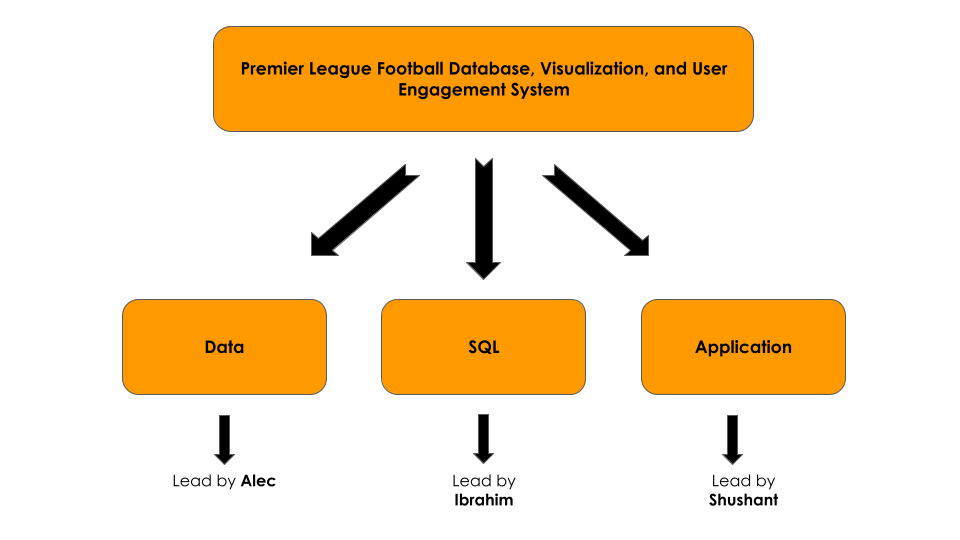
\includegraphics[width=1\linewidth]{Untitled presentation (3).png}
    \caption{Labor Division}
    \label{fig:enter-label}
\end{figure}

\begin{figure*}[ht]
\centering
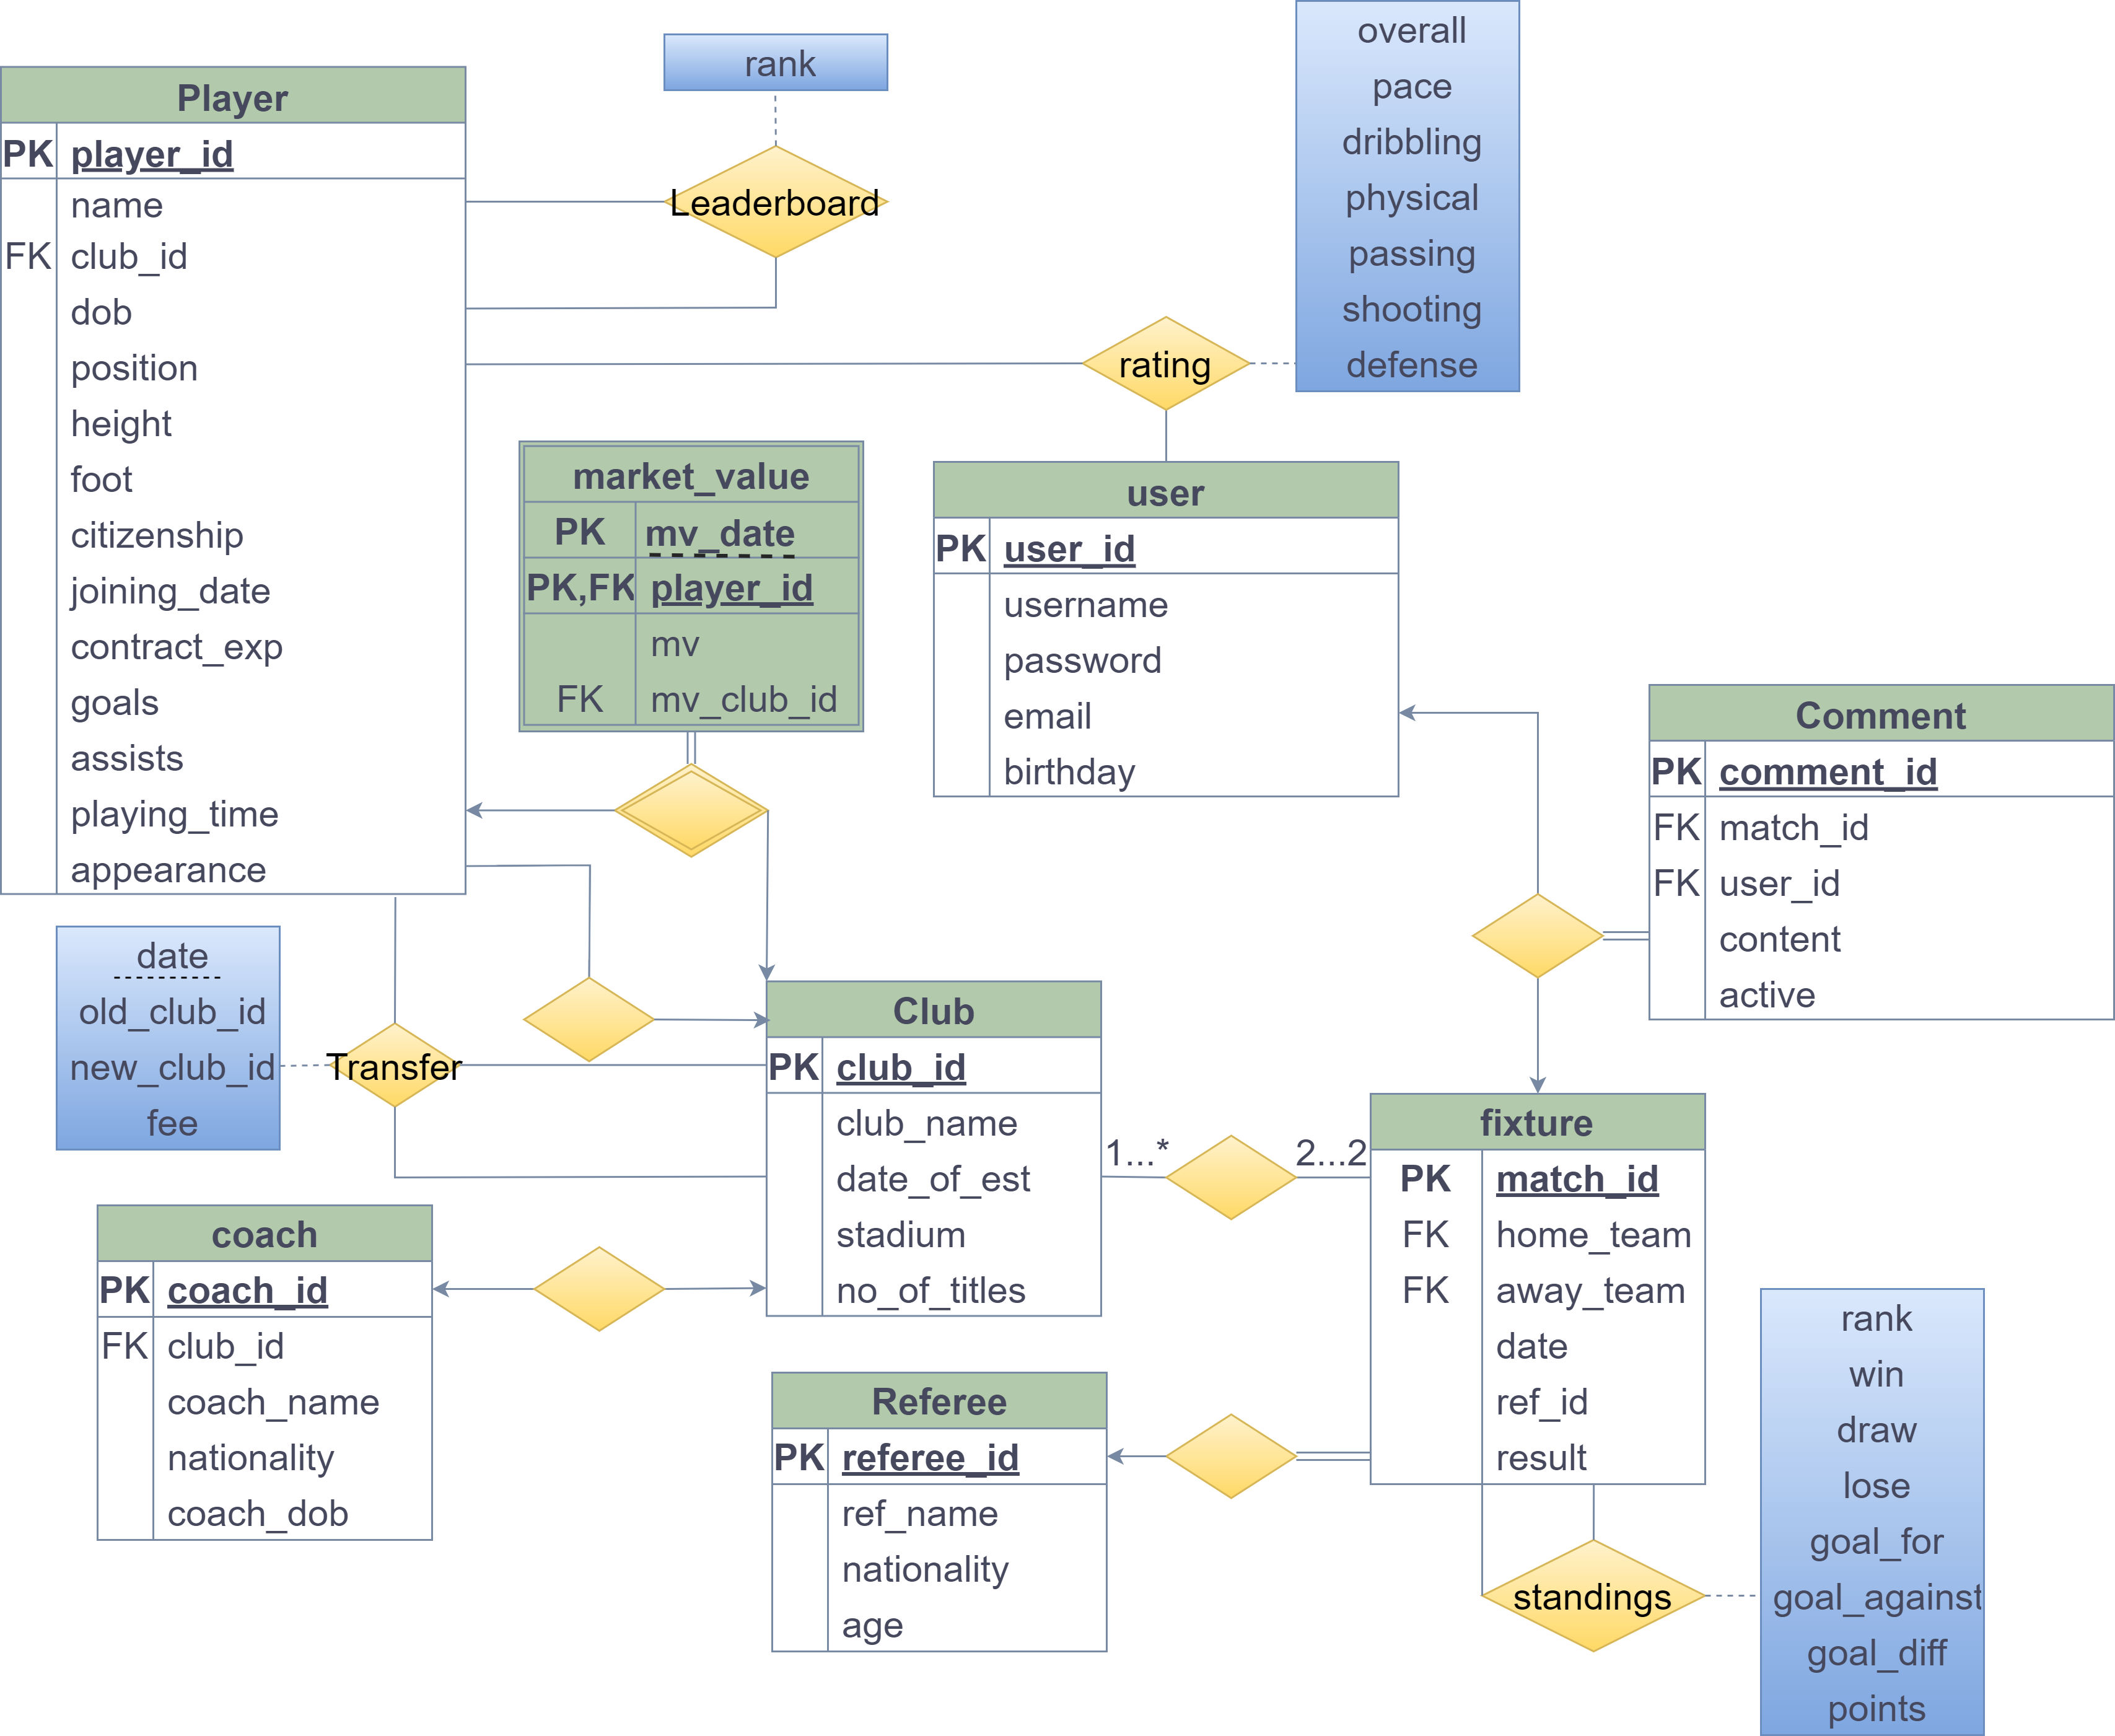
\includegraphics[width=0.9\textwidth]{New.drawio (1).png}
\caption{Final ERD}
\label{fig:yourlabel}
\end{figure*}
\section{Database Design}




\textit{Figure 2 represents the ERD of the Project}
\noindent \textbf{The database comprises various entities: }



\begin{itemize}
    \item \textbf{Player}: This entity stores basic player information and performance statistics. 
    \item \textbf{Market\_Value}: Contains historical market values of players, along with the clubs they were affiliated with at those times. 
    \item \textbf{Club}: Represents football clubs. 
    \item \textbf{Coach}: Details of each club's head coach. 
    \item \textbf{Fixture}: Acts as the match table. 
    \item \textbf{Referee}: Information about match referees. 
    \item \textbf{User}: Users of the database system. 
    \item \textbf{Comment}: User-generated comments on specific matches. 
\end{itemize}
The relationships between these entities are defined as follows: 

\begin{itemize}
    \item A \textbf{Player} is associated with one club but can have multiple entries in the market\_value table, representing different market values at various clubs. Players can also have multiple transfer records, reflecting moves between clubs. They compete with each other, and the top 15 goal-scorers are featured on a leaderboard. We used player names as the primary key here since duplicated full names are extremely rare in one football league.
    \item Each \textbf{Club} is led by one head coach, and each coach is linked to a single club. Clubs participate in numerous matches. 
    \item A \textbf{Fixture} involves two clubs, designated as home\_team and away\_team, and is overseen by a single referee. Aggregating data from the Fixture entity yields the Standings. 
    \item \textbf{Users} can rate multiple players and post comments on various matches. While not every player may have a rating, and not every match might have comments, each comment is linked to a specific user and pertains to a particular match. 
\end{itemize}
All tables are normalized to at least 3NF. For instance, we excluded names whenever ids were stored, and we deleted ages since we had date of birth records. \\

\noindent\textbf{Schemas of the database are as follows:} 

\begin{itemize}
    \item \noindent \textbf{club\_final} (\underline{club\_id}, club\_name, date\_of\_est, no\_of\_titles, stadium);
    \item \noindent \textbf{coaches\_final} (\underline{coach\_id}, club\_id, coach\_name, nationality, coach\_dob);
    \item \noindent \textbf{comments\_final} (\underline{comment\_id}, user\_id, match\_id, content, isActive);
    \item \noindent \textbf{fixtures} (\underline{match\_id}, home\_team, away\_team, date, result, ref\_id);
    \item \noindent \textbf{hist\_final} (\underline{player\_id}, \underline{date}, old\_club\_id, new\_club\_id, fee);
    \item \noindent \textbf{leaderboard} (\underline{name}, goals, rank);
    \item \noindent \textbf{mv\_final} (\underline{player\_id}, mv\_date, mv, mv\_club\_id);
    \item \noindent \textbf{players\_final} (\underline{player\_id}, name, club\_id, dob, position, height, foot, citizenship, joining\_date, contract\_exp, goals, assists, playing\_time, appearance);
    \item \noindent \textbf{ratings\_final} (\underline{player\_id}, \underline{user\_id}, Overall, Pace, Shooting, Passing, Dribbling, Defense, Physical);
    \item \noindent \textbf{ref} (\underline{ref\_id}, ref\_name, dob, nationality);
    \item \noindent \textbf{standings\_final} (\underline{club\_id}, rank, win, draw, lose, goal\_for, goal\_against, goal\_diff, points);
    \item \noindent \textbf{users} (\underline{user\_id}, username, password, email, birthday)
\end{itemize}
\noindent\textbf{Table Summary:\\} 

%\begin{figure}
    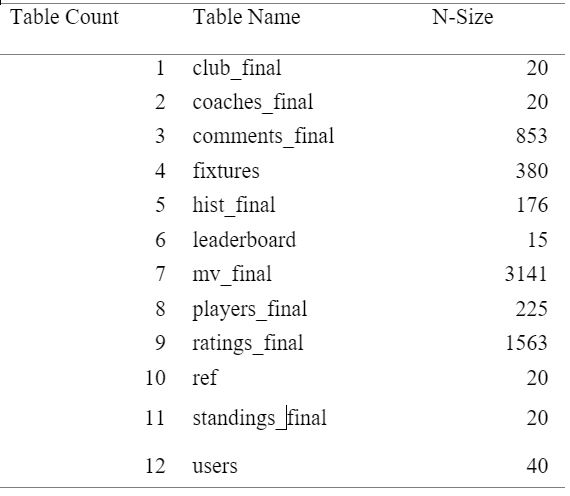
\includegraphics[width=1\linewidth]{table summary.jpg}

%\end{figure}

\section{Data Collection}
\noindent The data source of our database consists of Transfermarkt.com, FC24 (EA Sports FC 24), the Premier League official website, public information, and ChatGPT 4.0. 

The original data for the datasets \textit{players\_final}, \textit{hist\_final}, and \textit{mv\_final} was obtained by scraping information from \textbf{transfermarkt.com}\footnote{Transfermarkt. (2023). Retrieved Jan 01, 2023, from https://www.transfermarkt.com} using \textbf{Scrapy 2.5.1}\footnote{Scrapy Developers. (2022). Scrapy (Version 2.5.1) [Software]. Available from https://scrapy.org/} during the period from December 27, 2022, to January 01, 2023. The players included in\textit{ hist\_final}, \textit{mv\_final}, and the basic player information within \textit{players\_final} were those who participated in the 2022-23 season. Meanwhile, the player statistics data (e.g., goals and appearances) in players\_final pertained to players from the 2017-18 season. Typically, each Premier League season features more than 400 players. After filtering the datasets to include only players present in all three datasets with well-formatted information, we arrived at a final set of 225 players across \textit{players\_final}, \textit{hist\_final}, and \textit{mv\_final}. Original datasets for \textit{hist\_final} and \textit{mv\_final} contained information when players were not serving Premier League teams. Since they were not the focus of our design, market value and transfer records when players were serving other teams were removed from our final datasets. 

Data for the \textit{club\_final }and \textit{coaches\_final} datasets also originated from Transfermarkt.com, but these data were collected manually. In total, 20 clubs that played in the Premier League in season 2021-22 and their respective coaches were included. The \textit{leaderboard} was generated based on the cumulative number of goals scored by the 225 players up to the date when the data was scraped. 

The data for the \textit{fixtures} table consists of real matches from the 2022-23 season, which were scraped using the requests library from the \textbf{Premier League official website}. \footnote{Transfermarkt. (2023). Results. Retrieved Nov 15, 2023, from https://www.premierleague.com/results?co=1\&se=489\&cl=-1}. To make the data more reflective of reality, all match results after December 01, 2022 were removed, representing 'upcoming matches.' Additionally, all dates were adjusted by one year to align with the current ongoing season. The fixtures dataset comprises a total of 380 matches, with results available for 146 matches, while the remaining 234 matches are designated as 'upcoming matches.' 

The data for 20 referees was collected from publicly available sources, and their assignments to officiate matches were generated randomly. 

The \textit{standings\_final} dataset was derived from the 146 matches that had results. Using the match outcomes, we calculated each team's total points and other performance statistics. The teams were then ranked based on total points (in descending order), total number of matches (in ascending order), and goal differences (in descending order) to create the final standings. 

The \textit{users} and \textit{comments\_final} datasets were generated using \textbf{ChatGPT 4.0}\footnote{OpenAI. (2023). ChatGPT 4.0.}. User-related information, including usernames, passwords, emails, and birthdays, was created with the following prompts: 

"Generate 40 usernames for an England football forum." 

"Here is a list of usernames. Can you generate one password for each of them? Please return only the passwords." [List of generated usernames] 

"Here is a list of dummy usernames. Can you generate one email and one birthday for each of them? Please return only the emails and birthdays." [List of generated usernames] 

The contents of user comments were generated through the following prompt and subsequent iterations, as ChatGPT generates comments for a maximum of 10 games at a time: 

"Generate 6 short comments for the 146 football matches in the Premier League. Do not include any team names or player names. Please return the comments for ten games each time. Format your answers like Game 01: comment 1 comment 2 ..." 

Following the generation of six comments for each of the 146 matches with available results, one user was randomly assigned as the owner of each comment. Column \textit{isActive} shows if the owner account of the comment is active. 

The data in the \textit{ratings\_final} dataset was sourced from values obtained through web scraping at \textit{https://www.fifaratings.com/}. Initially, we collected ratings for players in \textbf{FC24}\footnote{FIFARatings. (2023). FC 24 Ratings Database. Retrieved Nov 14, 2023, from https://www.fifaratings.com/}, representing each player's attributes with a single value for each attribute. Subsequently, for each player, a randomized selection of 4 to 10 dummy users was made to provide ratings. These ratings were assigned random values within a range based on FC24 values, with an allowance of ±4. The rationale behind generating multiple ratings for each player was twofold: to simulate real-world rating systems and to mitigate the sensitivity of ratings to additional individual assessments. 


\section{Application Description}
\noindent\textbf{The main features of the Application include the use of 5 Views, 4 Stored Procedures, 3 Functions, and 1 Trigger as listed below:}  
\newline
\newline
\textbf{Views:} 

\begin{itemize}
    \item \textit{Club Standings :} A table containing the Club Standings for the current season.
    \item \textit{Fixtures : }A view to display the fixtures of the current week.
    \item \textit{Market Value :} A LineGraph representing the market value history of the selected player.
    \item \textit{Upcoming Fixtures : }A Timeline chart to show the Logos of teams playing the selected club.
    \item \textit{Players view : }A table showing the Players of the selected club and their basic Information.
\end{itemize}

 \noindent\textbf{Stored Procedures:} 

\begin{itemize}
    \item \textit{LogIn :} A stored procedure containing if-else statements to handle different cases when a new user logs in, a pre-existing user logs in, or a deleted user recovers their account.
    \item \textit{Inserting Comment :} A stored procedure to insert a comment and also check if the current user only posts once.
    \item \textit{Update Comment : }A stored procedure that manages to update a comment and verify if the change comes from the owner of the comment.
    \item \textit{Delete Comment :} A stored procedure that manages to delete a comment and verify if the change comes from the owner of the comment.
\end{itemize}

 \noindent\textbf{Functions:} 

\begin{itemize}
    \item \textit{Player Rating : }A scalar function calculating a player's rating based on the player's skill stats.
    \item \textit{Player Style :} A function to determine a player's playing style factoring in his skill sets.
    \item \textit{Match Count : }A function to determine the number of matches played by each club from the Fixtures table.
\end{itemize}

\noindent\textbf\textbf{Trigger:} 

\begin{itemize}
    \item \textit{User Deletion : }A trigger to update the Comments to inactive for a user in the comment table whenever a user is deleted from the User Table.
\end{itemize}



\begin{figure}[H]
    \centering
    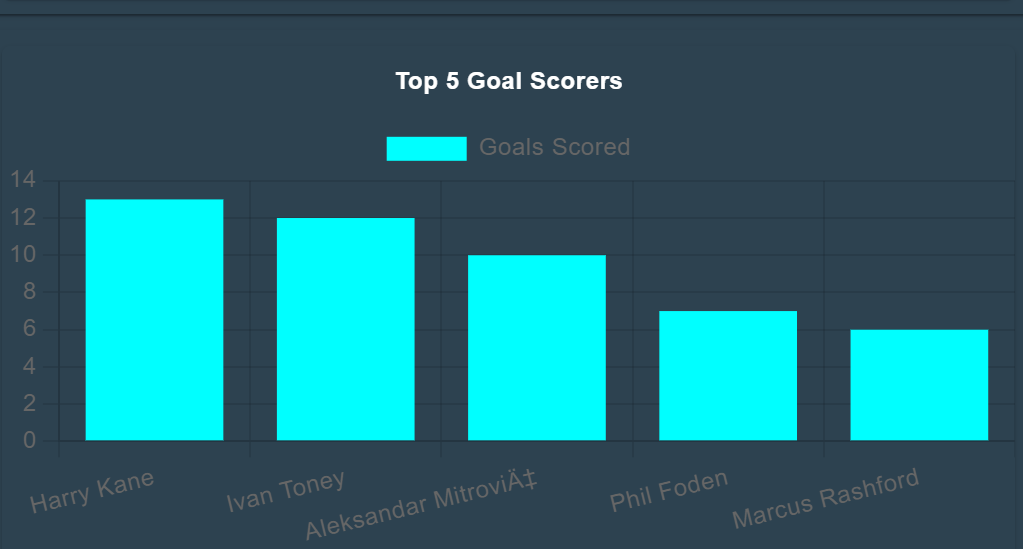
\includegraphics[width=0.9\linewidth]{Screenshot 2023-12-11 182720.png}
    \caption{Analytics 1}
    \label{fig:enter-label}
\end{figure}


\begin{figure}[H]
    \centering
    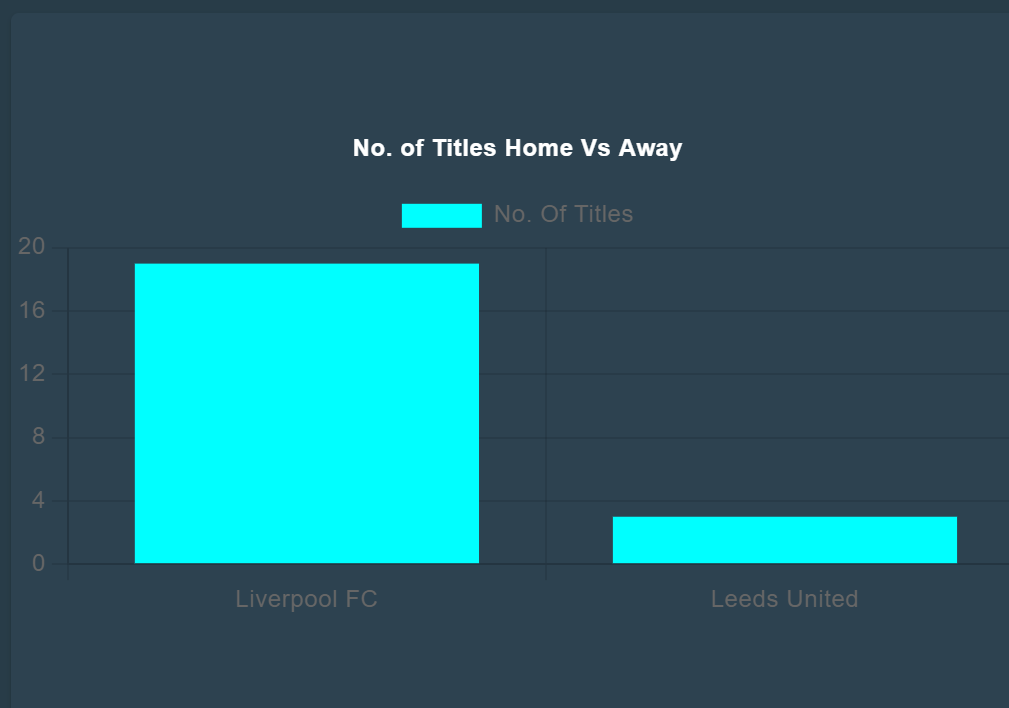
\includegraphics[width=0.9\linewidth]{Screenshot 2023-12-11 182745.png}
    \caption{Analytics 2}
    \label{fig:enter-label}
\end{figure}

%\begin{figure}
\begin{figure}[H]
    \centering
    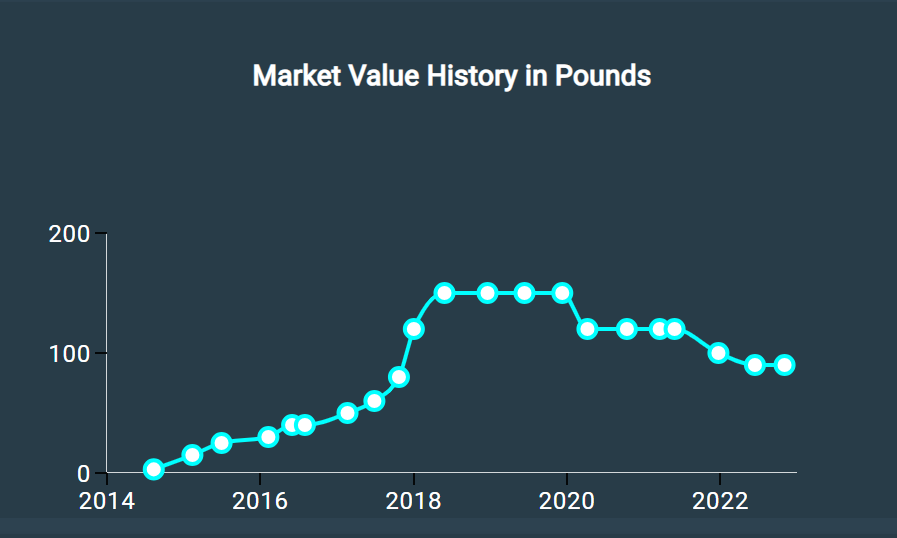
\includegraphics[width=0.9\linewidth]{Screenshot 2023-12-11 182807.png}
    \caption{Analytics 3}
    \label{fig:enter-label}
\end{figure}



\noindent\textbf{Analytics:} 

\begin{itemize}
    \item \textit{Top Scorer Bar Chart : }A Bar Chart displaying the Top-5 Goal scorers for the season.\textit{Fig 3}

    \item \textit{League Titles BarChart :} A comparative analysis between two clubs based on the no. Of League titles won.\textit{Fig 4}

    \item \textit{Market Value LineGraph :} A Linegraph displaying the a Players historical Market Values.\textit{Fig 5}

\end{itemize}

\noindent The Storing and retrieval of Data From the UI to the MySQL database can be understood from \textit{Figure 7}. \\ \\


\noindent We used \textbf{Axios} for our \textbf{GET} and \textbf{POST} calls from the \textbf{ReactUI} to\textbf{ python backend} and then using \textbf{mysql-connector} we established a connection with the \textbf{MySQL DB} and stored and Retrieved Data. An example of the connection establishment and Data retrieval using Python can be seen in \textit{Figure 6}.

\begin{figure}[H]
    \centering
    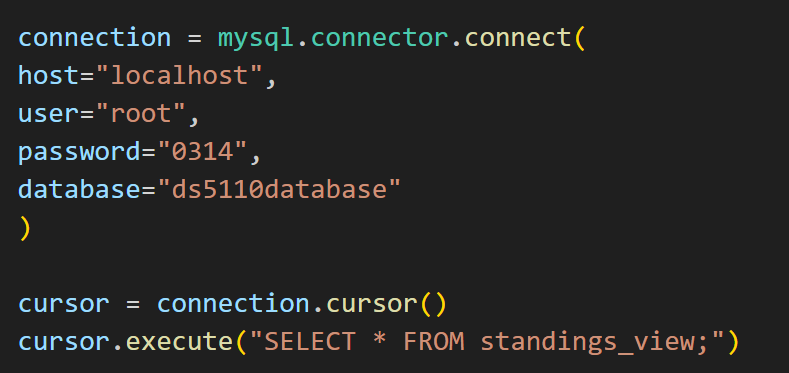
\includegraphics[width=0.9\linewidth]{Screenshot 2023-12-10 113221.png}
    \caption{Sample Data Retrieval}
    \label{fig:enter-label}
\end{figure}


\begin{figure}[H]
    \centering
    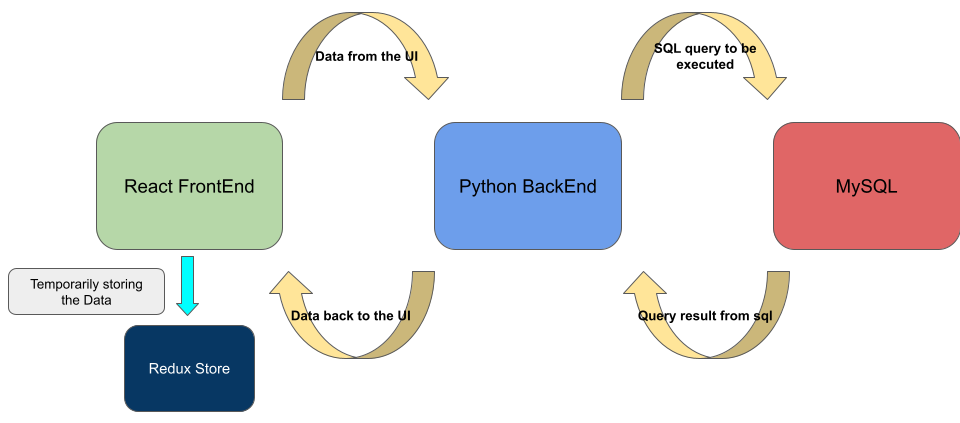
\includegraphics[width=0.9\linewidth]{Untitled presentation (2).png}
    \caption{Data Storage and Retrieval}
    \label{fig:Data}
\end{figure}

\section{Conclusion}

This project successfully demonstrates the utilization of proper database design procedures and various methodologies to create a Premier League Data Management and Visualization Application. The system's user-friendly interface, robust data management capabilities, and interactive features make it an engaging and informative platform for both casual and dedicated fans. 

In our project, we extensively practiced various aspects of SQL database management, web scraping, and the transfer of information between the front end and back end. If given more time, we would aim to enhance our project in the following key areas:
\begin{itemize}
    \item \textbf{Introduce functionality for users to rate players}, transitioning from a static/read-only format (as per the current version) to a more dynamic and interactive feature. 
    \item \textbf{Display transfer history information}, possibly on dedicated player pages, offering a more comprehensive view of each player's journey. 
    \item \textbf{Employ machine learning or statistical methods} to predict market values of players, adding a predictive dimension to our analytical functionality. 
    \item \textbf{Integrate an admin user role}, endowed with the authority to upload new match details and update player statistics, ensuring our database remains current and accurate. 
    \item \textbf{Develop a sign-up page} that collects user demographics and credentials, such as email addresses and passwords. This addition would enhance user engagement and provide the foundation for user account security measures.
\end{itemize}

\textbf{Future students} undertaking a project like the Premier League Database and User Engagement System should prioritize two key principles: \textbf{robust database design }and\textbf{ a user-centric approach}. Stress the importance of efficient database structuring for optimal data management, while also encouraging the incorporation of dynamic features to enhance the user experience. Emphasize continual improvement by considering future enhancements such as predictive analytics, admin user roles, and enhanced security measures. Additionally, underscores the real-world relevance of the project by applying database design and data transfer in practical contexts like sports. Advocate for thorough documentation, effective team communication, and efficient time management to ensure successful project outcomes that not only meet current needs but also allow for future enhancements.
 





\end{document}